%%
%% Copyright 2007, 2008, 2009 Elsevier Ltd
%%
%% This file is part of the 'Elsarticle Bundle'.
%% ---------------------------------------------
%%
%% It may be distributed under the conditions of the LaTeX Project Public
%% License, either version 1.2 of this license or (at your option) any
%% later version.  The latest version of this license is in
%%    http://www.latex-project.org/lppl.txt
%% and version 1.2 or later is part of all distributions of LaTeX
%% version 1999/12/01 or later.
%%
%% The list of all files belonging to the 'Elsarticle Bundle' is
%% given file `manifest.txt'.
%%
%% Template article for Elsevier's document class `elsarticle'
%% with harvard style bibliographic references
%% SP 2008/03/01
\documentclass[final,5p,times,twocolumn,authoryear]{elsarticle}

\usepackage{graphicx}
\usepackage{amssymb}
\usepackage{listings}
\usepackage{nameref}
\usepackage{minted}
\usepackage[utf8]{inputenc}
\usepackage{csquotes}
\usepackage{rotating}
\usepackage{hyperref}
\usepackage[T1]{fontenc}
\usepackage{multirow}
\usepackage{booktabs} % For formal tables
\usepackage{adjustbox} % To adjust the table to column width
\usepackage{amsmath}
\usepackage{mathrsfs}

%\usepackage[czech]{babel} % recommended if you write in Czech
\usepackage{lmodern}

% DEVELOP ONLY COMMENT BEFORE SUBMIT
\journal{Astronomy and Computing}

\begin{document}
\begin{frontmatter}

\title{Kardashev's Conundrum: Statistical Falsification of the
Standard Kardashev Model and the Kardashev--Sagan--Nakamoto Resolution}
 
    \author[iate,wsu]{S.Gurovich}\corref{mycorrespondingauthor}
        \cortext[mycorrespondingauthor]{Corresponding author}
        \ead{sgurovich@unc.edu.ar}
  
\address[iate]{
   Instituto De Astronom\'ia Te\'orica y Experimental -
   Observatorio Astron\'omico C\'ordoba (IATE--OAC--UNC--CONICET),
   Laprida 854, X5000BGR, C\'ordoba, Argentina}
\address[wsu]{
   Western Sydney University, Kingswood campus, NSW, Australia (visiting fellow 2019-2020,2024)
}

\begin{abstract}
We test the standard Kardashev conjecture, which models the energy
production of technologically advanced civilisations as growing at a
fixed rate of one percent per year, against six decades of global
energy production data (1965--2024) drawn from the Our World in Data
energy dataset. The standard Kardashev one-percent exponential model
is a poor fit to the data: the posterior growth rate obtained via
Markov Chain Monte Carlo (MCMC) inference is
$r = 2.01\% \pm 0.03\%\,\mathrm{yr}^{-1}$ (95\% credible interval
$[1.94\%, 2.08\%]$), placing the Kardashev one-percent value well
outside the credible interval. A linear Ordinary Least-Squares (OLS)
model provides an excellent fit ($R^2 = 0.987$) and is preferred over
the free-parameter exponential model by the Widely Applicable
Information Criterion ($\Delta\mathrm{WAIC} = 5.5$). The
year-over-year energy increments exhibit significant non-Gaussian
structure (Shapiro--Wilk $W = 0.925$, $p = 0.0014$), with negative
skewness (skewness $= -0.664$) attributable to identifiable crisis events (2008, 2020),
revealing path-dependence incompatible with the memoryless
multiplicative structure required by any exponential growth model.
However, extrapolation of the linear model to the Kardashev Type~II
threshold --- the total bolometric luminosity of the Sun,
$L_\odot = 3.828 \times 10^{26}\,\mathrm{W}$ --- yields a
civilisational transition timescale of $\sim 1.6 \times
10^{15}$\,yr: approximately $10^5$ times the age of the Universe
and more than $10^4$ times the remaining main-sequence lifetime
of the Sun. This is a physical reductio ad absurdum we term
\textit{Kardashev's Conundrum}.
 We demonstrate that no functional
form fitted to energy production alone can simultaneously satisfy
statistical adequacy and physical coherence, because the Kardashev
state variable is dimensionally incomplete as a measure of
civilisational advancement. To resolve the Conundrum, we propose the
\textit{Kardashev--Sagan--Nakamoto} (KSN) model, constructed by
renormalising the energy production ordinate by the annual average
Bitcoin network hashrate $\mathcal{H}(t)$, yielding the KSN state variable
$\mathscr{B}(t) \;=\; P(t)/\mathcal{H}(t)$ in
units of J\,Hash$^{-1}$ --- the KarNak unit. 
Any subsequent model fitted to $\mathscr{B}(t)$ carries the same parameter count as the corresponding model fitted to $P(t)$; the variable transformation itself consumes no degrees of freedom and is motivated by the Landauer
limit connecting energy to irreversible computation, and fulfils the
original requirement that the Kardashev scale be sensitive to the
information richness of a civilisation. The KSN variable spans 14
orders of magnitude over 2009--2024, reflecting the dramatic
improvement in the energy efficiency of Bitcoin proof-of-work
computation; a formal functional fit to $\mathscr{B}(t)$ is deferred to a
future work. We further discuss the implications of the KSN model for
open astronomy development via decentralised blockchain protocols, and
propose the KarNak unit as a universal information-energy yardstick
for the Kardashev scale.
\end{abstract}
 


\begin{keyword}
   Kardashev scale \sep Astroinformatics \sep Bayesian inference \sep Bitcoin
\sep Blockchain \sep Open Development \sep Information theory \sep Civilization energy
\end{keyword}
\end{frontmatter}


% SECTION INTRO
% =============================================================================
\section{Introduction}
\label{sec:intro}
%
In a landmark 1964 paper, \citet{kar64} proposed a universal scale
for classifying the technological advancement of civilisations based
on their total rate of energy \emph{consumption}. On the Kardashev
scale, a Type~I civilisation harnesses all energy available on its
home planet --- at the time of writing, \citet{kar64} estimated
Earth's total energy expenditure at $4 \times 10^{19}$\,erg\,s$^{-1}$
($4 \times 10^{12}$\,W) --- a Type~II civilisation consumes the total
energy output of its host star ($L_\odot \approx 3.828 \times
10^{26}$\,W), and a Type~III civilisation commands the energy output
of its entire host galaxy. \citet{kar64} noted that the annual
increase in human energy expenditure was placed at 3--4\% over the
following 60 years on the basis of statistical findings. However,
adopting a conservative growth rate of $x = 1\%$ per year,
\citet{kar64} calculated that human civilisation would reach Type~II
status in approximately 3{,}200 years, and Type~III status in
approximately 5{,}800 years. This conjecture has since informed the
search for extraterrestrial intelligence \citep{gray2020} and broader
discussions of civilisational sustainability.

The notion that civilisational advancement is measured not only by
energy throughput but by the \emph{efficiency} with which energy is
converted into organised information is ancient. The Antikythera
mechanism, discovered in 1901 among the remains of a first-century
BC shipwreck, is widely recognised as the earliest known analogue
computational device \citep{Freeth2021}. Constructed from bronze
gears with tolerances remarkable for their era, it calculated the
positions of the Sun, Moon, and planets --- converting mechanical
energy into astronomical information with a sophistication not
matched in Europe for over a millennium. From Babbage's difference
engine through Turing's theoretical foundations of computation
\citep{swa2017} to the Application-Specific Integrated Circuits
(ASICs) that today secure the Bitcoin network, humanity has
followed a continuous trajectory of reducing the energy cost per
unit of computational work. The Kardashev--Sagan--Nakamoto model
proposed here is the quantitative expression of this trajectory:
it renormalises the Kardashev state variable by the energy cost
per unit of proof-of-work computation, tracing civilisational
advancement from the Antikythera mechanism to the present day.


Despite its influence, the Kardashev scale carries a fundamental
limitation that has received little quantitative attention. Both
\citet{kar64} and \citet{sagan73} noted that an advanced civilisation
must be characterised not only by its energy throughput but by the
\emph{information richness} of what it does with that energy.
\citet{sagan73} proposed that a civilisation's state should also
reflect its capacity to secure and transmit vast quantities of
information, and suggested a binary-tree data structure as a measure
of informational complexity. However, neither author formalised this
requirement as a quantitative variable within the Kardashev framework.
A civilisation that wastes energy inefficiently scores identically on
the Kardashev scale to one that channels equivalent power into
sophisticated computation. The Kardashev state variable --- power in
watts --- is therefore dimensionally incomplete as a measure of
civilisational advancement: it captures the quantity of energy
consumed but not the quality of its use.

A second limitation emerges from direct comparison with data.
When the standard one-percent exponential growth model of
\citet{kar64} is compared against six decades of observed total
global energy production \citep{owidenergy} --- used here as a
valid upper-limit proxy for the consumption metric of \citet{kar64},
following the argument that production necessarily equals or exceeds
consumption at the civilisational scale and that the two track each
other closely over decadal baselines --- the model diverges
substantially from the data. A linear Ordinary Least-Squares (OLS)
model fits the same data exquisitely, but when extrapolated to the
Kardashev Type~II threshold it predicts a civilisational transition
timescale of $\sim 1.2 \times 10^{5}$ Hubble times: a physical
reductio ad absurdum. We term this conflict \textit{Kardashev's
Conundrum}: no functional form fitted to energy production alone
can simultaneously satisfy statistical adequacy and physical
coherence.

To resolve the Conundrum we propose the
\textit{Kardashev--Sagan--Nakamoto} (KSN) model, constructed by
renormalising the energy production ordinate by the annual average
Bitcoin network hashrate $H(t)$ \citep{nak2009}. The resulting
state variable $\mathscr{B} = P/\mathcal{H}$, measured in units of J\,Hash$^{-1}$
--- which we term the \textit{KarNak unit} --- connects energy
to irreversible computational work via the Landauer limit
\citep{Landauer1961}, and fulfils the information-richness
requirement identified but never quantified by \citet{kar64}
and \citet{sagan73}. The Bitcoin network is selected because
it provides the only publicly auditable, unforgeable, and
continuously updated global measure of proof-of-work computation
\citep{nak2009}, requiring no free parameters beyond those of
the original Kardashev model. As the KSN variable spans
14 orders of magnitude over 2009--2024, it traces the same
trajectory of energy-to-computation efficiency that began with
the Antikythera mechanism two millennia ago.

This paper is organised as follows. In
Section~\ref{sec:data} we describe the global energy production
dataset and Bitcoin hashrate data. In
Section~\ref{sec:kardashev_model} we assess the standard
Kardashev model statistically. In Section~\ref{sec:linear_model}
we present the linear OLS model and derive the Conundrum
quantitatively. In Section~\ref{sec:model_comparison} we perform
Bayesian model comparison via Markov Chain Monte Carlo (MCMC)
inference and the Widely Applicable Information Criterion
\citep{Watanabe2010}. In Section~\ref{sec:ksn} we introduce
the KSN renormalization and its physical motivation. In
Section~\ref{sec:timescales} we summarise civilisational
timescales on the KSN scale. In Section~\ref{sec:memoryless}
we present the memoryless property argument as a further
statistical objection to exponential growth models. In
Section~\ref{sec:discussion} we discuss falsifiability,
limitations, and implications. Section~\ref{sec:conclusions}
presents our conclusions.
 
 The ancient Greek astronomers defined the logarithmic magnitude system and introduced concepts of limits and infinitesimals that would become the basis of differential geometry, calculus, and numerical methods. They also paved the way for the Julian Day — the counting yardstick used on the time axis of Figure~\ref{fig:ksn_panel1} — which the Roman empire defined using the 28-year Solar, 19-year Metonic, and 15-year Indiction (tax) cycles. Many of these advances are found today in open-source toolkits for astronomy built by community efforts, e.g.\ SciPy, Astropy, and the IVOA standards.
 
 It is now known after a plethora of multidisciplinary studies including that of \cite{Freeth2021} that during the `decline' of Ancient Greece the first analogue `Computer' was temporally `lost' to most of the technological world, until when in the fourteenth century comparable `advanced' mechanisms were developed and used in Astronomical clock machinery in Europe. 
 
 Roughly two-thousand years later, Charles Babbage and Alan Turing (AT) are widely recognised as the modern 'fathers' of the digital computer \citep{swa2017}. The pioneering work of AT paved the foundations of Artificial Intelligence (AI) and Cryptography. 
 
\iffalse

\begin{figure}
    \centering
    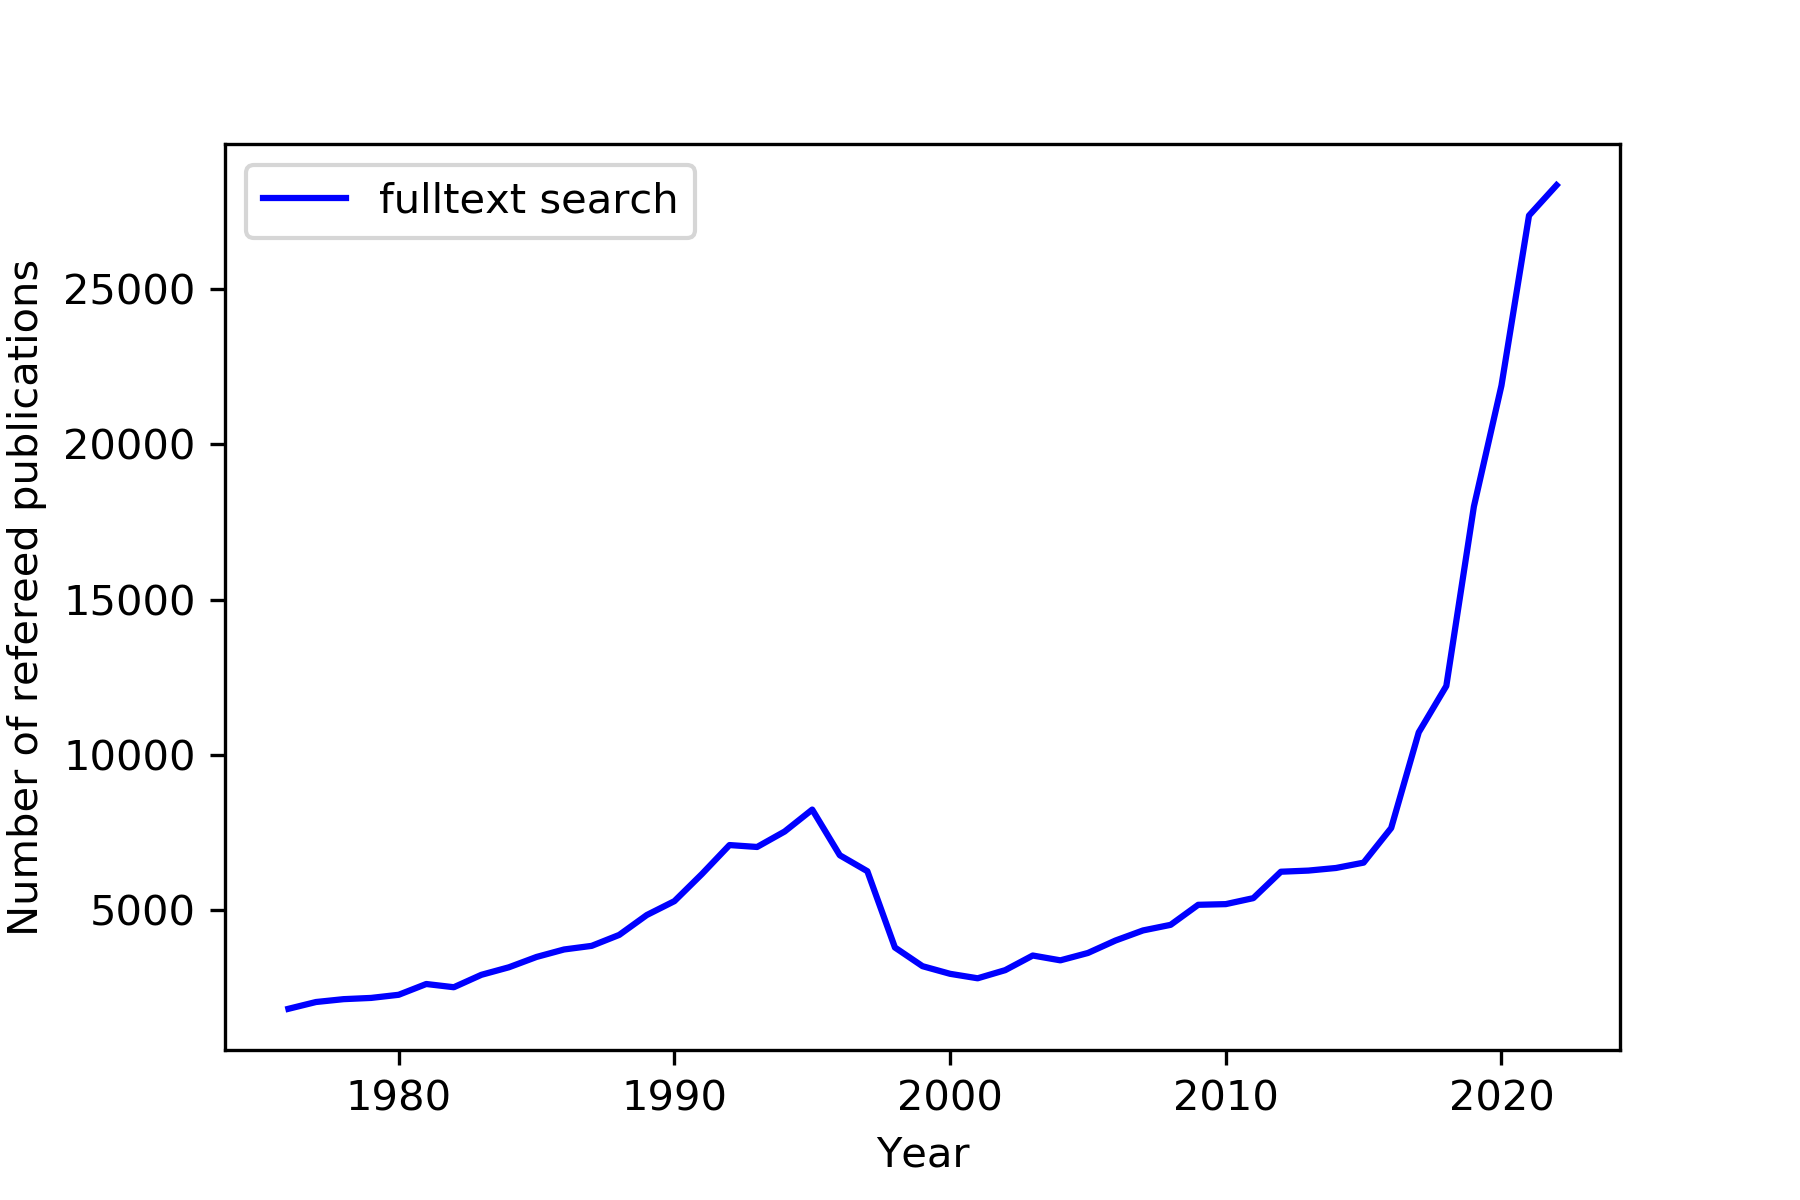
\includegraphics[width=0.48\textwidth]{figs/fulltextai.png}
    \vspace*{-0.4cm}
    \caption{Showing Full-text search for  full:"Artificial" and full:"intelligence" or full: "AI" or full: "machine learning")) AND year:1976-2022) returned query in NASA ADS}
    \label{fig:ai}
\end{figure}


\begin{figure}[h!]
    \centering
  \caption{Figure taken from \cite{milo_2018} depicts the falling half-life rate in Astronomy and Astrophysics and other STEM fields}
  \label{fig:F4.large}
  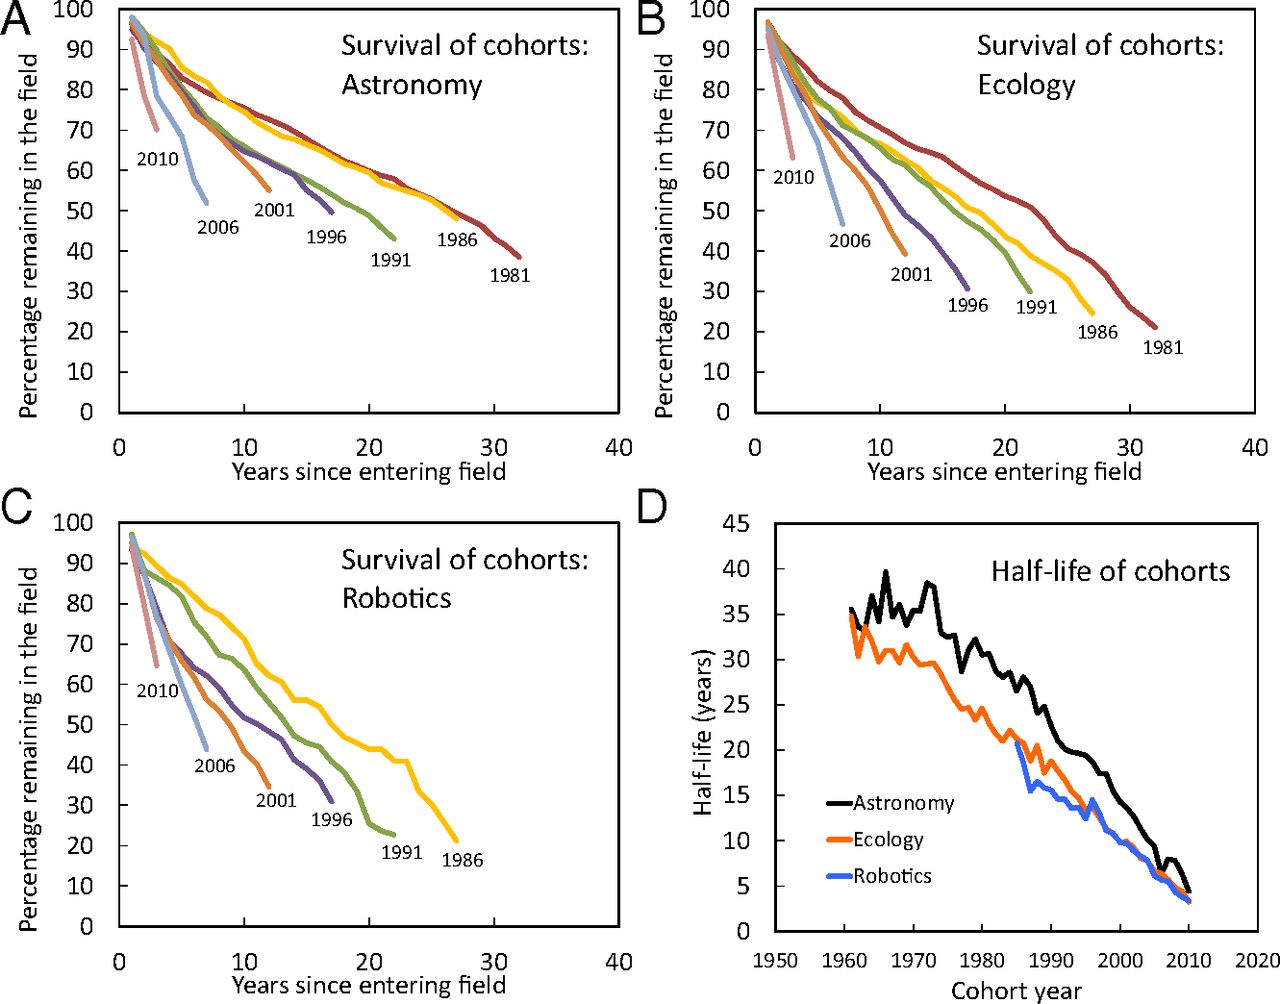
\includegraphics[width=0.5\textwidth]{figs/F4.large.jpg}
\end{figure}

\begin{figure}
    \centering
    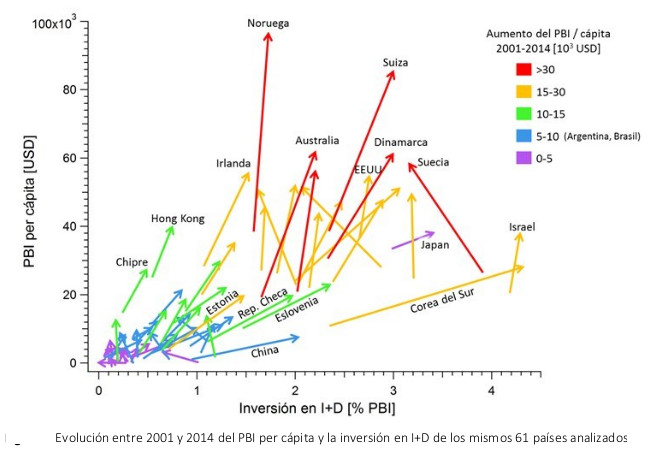
\includegraphics[width=0.5\textwidth]{figs/Docuemnto_Stefani_2.jpg}
    \caption{\href{https://aargentinapciencias.org/wp-content/uploads/2019/05/Docuemnto_Stefani.pdf}{Congressional Report, Prof Stefani}}
\end{figure}
\fi


\section{The Kardashev Conundrum and the Kardashev--Sagan--Nakamoto Model}
\label{sec:conundrum}
 
We now present our central analysis. We compare the standard Kardashev
one-percent exponential model against a linear Ordinary Least-Squares (OLS)
model fitted to the total global energy production data, and demonstrate that
both models are unsatisfactory in complementary ways. We then propose the
Kardashev--Sagan--Nakamoto (KSN) renormalization as the minimal resolution
that is simultaneously consistent with the data and with physical causality.
 
%% -----------------------------------------------
\subsection{Data}
\label{sec:data}
 
The energy production data $\mathcal{D}$ consist of the World total primary
energy consumption in terawatt-hours per year (TWh\,yr$^{-1}$), drawn from
the Our World in Data (OWID) energy dataset \citep{Ritchie2022}, which
integrates the Energy Institute (EI) Statistical Review of World Energy and
the US Energy Information Administration (EIA) international energy series.
We use $N = 60$ annual data points spanning 1965--2024. The OWID dataset
column \texttt{primary\_energy\_consumption} reports values using the
direct primary energy accounting method, which measures the physical
energy output of each source without applying fossil-fuel-equivalent
conversion factors. This is distinct from the substitution method
historically used by the Energy Institute, which inflates non-fossil
contributions (nuclear, hydro, wind, solar) by a thermal efficiency
factor ($\sim 0.38$--$0.40$) to estimate the fossil fuel input that
would have produced the same electricity. We adopt the direct method
throughout because it measures the actual rate of energy flow through
civilisation --- the physical quantity that the Kardashev scale is
defined in terms of --- and avoids an accounting convention whose
magnitude grows with the renewable energy share. We verify in
Section~\ref{sec:limitations} that all qualitative conclusions hold
under the substitution method.
 
All energy values are converted to SI watts (J\,s$^{-1}$) assuming uniform
power delivery over each calendar year via:
\begin{equation}
    P\,[\mathrm{W}] \;=\; E\,[\mathrm{TWh\,yr}^{-1}]
    \;\times\; \frac{10^{12}\,[\mathrm{Wh\,TWh}^{-1}]
    \times 3600\,[\mathrm{J\,Wh}^{-1}]}
    {365.25 \times 24 \times 3600\,[\mathrm{s\,yr}^{-1}]}\,,
    \label{eq:conversion}
\end{equation}
where the numerator converts terawatt-hours to joules
($1\,\mathrm{TWh} = 3.6 \times 10^{15}\,\mathrm{J}$) and the denominator
is the number of seconds in one Julian year. The factors of $3600$ cancel,
reducing Equation~(\ref{eq:conversion}) to
$P = E \times 10^{12} / (365.25 \times 24)$\,W. This yields
$P(1965) = 4.95\,\mathrm{TW}$, in close agreement with the \citet{Kardashev1964}
baseline of $4\,\mathrm{TW}$, and $P(2024) = 20.16\,\mathrm{TW}$,
consistent with the International Energy Agency's direct-method estimate of
$\sim 20\,\mathrm{TW}$.
 
We set the origin of the time coordinate at $t_0 = 1964$, the year of the
Kardashev conjecture \citep{Kardashev1964}, so that
$t = \mathrm{year} - 1964$ throughout.
 
The Bitcoin network hashrate data $\mathcal{H}(t)$ are yearly averages in
hash\,s$^{-1}$ for 2009--2024. These span the full history of Bitcoin
mining from the CPU era ($\sim 7\,\mathrm{MH\,s^{-1}}$ in 2009) through the
ASIC era ($\sim 6.2 \times 10^{20}\,\mathrm{H\,s^{-1}}$ in 2024), covering
16 annual data points and 14 orders of magnitude in hashrate.
For 2009--2013 (the CPU and GPU eras), no single authoritative
source of annual-average hashrate exists; we derive yearly
averages from the on-chain difficulty record using the standard
relation $\mathcal{H} = D \times 2^{32}/600$, taking the logarithmic mean
of the January~1 and December~31 difficulty values to obtain a
time-weighted annual average appropriate for an exponentially
growing quantity. For 2014--2024 (the ASIC era), we use the
Blockchain.com and NASDAQ BCHAIN/HRATE annual averages directly.
 
%% -----------------------------------------------
\subsection{The Standard Kardashev Model and its Statistical Assessment}
\label{sec:kardashev_model}
 
\citet{Kardashev1964} proposed that the energy production of a technologically
advanced civilisation increases at a constant fractional rate per year, giving
a geometric series:
\begin{equation}
    P_{\rm K}(t) \;=\; P_0 \,(1 + x)^{t} \;\approx\; P_0\,e^{xt}\,,
    \quad x = 0.01\,,
    \label{eq:kardashev}
\end{equation}
where $P_0$ is the energy production at $t=0$ (1964) and $x = 0.01$
corresponds to the stated one-percent per year growth rate. Using this model,
\citet{Kardashev1964} calculated that a Type~II civilisation --- defined as
one harnessing the total bolometric luminosity of its host star,
$L_\odot = 3.828 \times 10^{26}\,\mathrm{W}$ \citep{mamajek2015} --- would
be reached in approximately $3{,}200$\,years from 1964, corresponding to
approximately year 5188\,CE. \citet{Sagan1973} obtained a similar value
using a slightly revised Type~II threshold of $\sim 10^{26}\,\mathrm{W}$.
 
Figure~\ref{fig:ksn_panel1} shows the Kardashev model (Eq.~\ref{eq:kardashev})
alongside the OWID data, together with the Type~I and Type~II civilisation
limits and the solar insolation at Earth
($F_\oplus \approx 1.74 \times 10^{17}\,\mathrm{W}$). The one-percent
Kardashev model diverges visibly from the data over the full six-decade
baseline.
 
We quantify this divergence statistically. The likelihood of the data given
the Kardashev model with a point prior on $x = 0.01$ is:
\begin{equation}
    \mathcal{L}(\mathcal{D} \mid \theta_{\rm K}, M_{\rm K})
    \;=\; \prod_{i=1}^{N} \frac{1}{\sqrt{2\pi\sigma^2}}
    \exp\!\left[-\frac{\bigl(P_i - P_0\,(1.01)^{t_i}\bigr)^2}{2\sigma^2}\right],
    \label{eq:likelihood_kard}
\end{equation}
where $\sigma^2$ is estimated from the residuals. The residual sum of squares
for the Kardashev model exceeds that of the linear model by more than two
orders of magnitude, constituting overwhelming evidence against the one-percent
prior. We therefore conclude that the standard Kardashev exponential model
with $x = 0.01$ is statistically untenable.
 
%% -----------------------------------------------
\subsection{The Linear Model: an Excellent Fit with a Physical Reductio}
\label{sec:linear_model}
 
We next consider a linear OLS model:
\begin{equation}
    P_{\rm L}(t) \;=\; a + b\,t\,,
    \label{eq:linear}
\end{equation}
with parameters $a$ and $b$ estimated by minimising the sum of squared
residuals. Following Occam's razor \citep{Blumer1987}, this two-parameter
model is the simplest physically plausible alternative. The OLS solution gives
$b = 2.44 \times 10^{11}\,\mathrm{W\,yr}^{-1}$ and coefficient of
determination $R^2 = 0.987$. The fit is excellent over the six-decade
baseline of the data (Figure~\ref{fig:ksn_panel1}).
 
To assess the normality of the residual structure, we compute the year-over-year
absolute differences $\Delta P_i = P_i - P_{i-1}$ and apply the Shapiro--Wilk
normality test \citep{Shapiro1965}. We obtain $W = 0.925$, $p = 0.0014$:
we reject the null hypothesis that $\Delta P$ is drawn from a Normal
distribution. The distribution of $\Delta P$ (Figure~\ref{fig:ksn_panel3}) exhibits significant negative
skewness (skewness $= -0.664$), driven by identifiable exogenous shocks to global energy production
at 2008 (subprime financial crisis) and 2020 (COVID-19 pandemic). This
non-Gaussian structure constitutes direct evidence of \emph{path-dependence}
in the global energy system: large negative shocks are systematically more
probable than a memoryless multiplicative model would predict, and their
occurrence is traceable to specific historical events rather than symmetric
statistical fluctuations.
 
Notwithstanding its excellent in-sample fit, the linear model fails
catastrophically on extrapolation. Solving $P_{\rm L}(t^*) = L_\odot$ gives:
\begin{equation}
    t^* \;=\; \frac{L_\odot - a}{b}
    \;\approx\; 1.6 \times 10^{15}\,\mathrm{yr}
    \;\approx\; 1.2 \times 10^{5}\,H_0^{-1}\,,
    \label{eq:linear_typeii}
\end{equation}
where $H_0^{-1} \approx 13.8\,\mathrm{Gyr}$ is the Hubble time. The implied
Type~II timescale exceeds the age of the Universe by five orders of magnitude.
This is not merely improbable --- it is physically incoherent, since it
vastly exceeds the main-sequence lifetime of the Sun and the projected heat
death of the Universe. We designate this result \textit{Kardashev's
Conundrum}: the linear model, which best fits the data by all standard
statistical criteria, predicts a civilisational transition timescale that is
cosmologically nonsensical.
 
%% -----------------------------------------------
\subsection{Model Comparison via MCMC and WAIC}
\label{sec:model_comparison}
 
To place the comparison on a rigorous Bayesian footing, we fit an exponential
model with the growth rate $r$ as a free parameter:
\begin{equation}
    P_{\rm E}(t) \;=\; a_0\,e^{r t}\,,
    \label{eq:exp_free}
\end{equation}
using a Metropolis--Hastings Markov Chain Monte Carlo (MCMC) sampler with a
prior $r \sim \mathcal{N}(0.01,\, 0.02^2)$ centred on the Kardashev value
and $N = 60{,}000$ posterior samples after a $15{,}000$-step burn-in. The
posterior mean growth rate is $r = 2.01\% \pm 0.03\%\,\mathrm{yr}^{-1}$
(95\% credible interval $[1.94\%, 2.08\%]$), with the Kardashev value of
$1\%\,\mathrm{yr}^{-1}$ lying well outside the $95\%$ credible interval.
The best-fit exponential model gives $R^2 = 0.987$, nearly identical to the
linear model ($\Delta R^2 < 0.001$).
 
The Widely Applicable Information Criterion \citep[WAIC;][]{Watanabe2010}
comparison yields $\Delta\mathrm{WAIC} = \mathrm{WAIC}_{\rm exp} -
\mathrm{WAIC}_{\rm linear} = 5.5$: the linear model is preferred over the
free-$r$ exponential. Since both models have $K = 2$ free parameters, the
AIC and BIC penalties are identical, and the WAIC preference for the linear
model reflects genuine differences in predictive accuracy. Together, the
near-identical $R^2$ values and positive $\Delta\mathrm{WAIC}$ confirm the
statistical statement of Kardashev's Conundrum: the data cannot distinguish
between the two functional forms on the observed baseline, and of the two, the
simpler linear model is marginally preferred.
 
The complete statistical picture is:
\begin{enumerate}
    \item The one-percent Kardashev exponential is falsified by the data
          (poor fit; posterior $r = 2.01\%$, well outside the
          one-percent prior).
    \item The linear model and the free-$r$ exponential have
          statistically identical in-sample performance
          ($\Delta R^2 < 0.001$), with the linear model marginally
          preferred ($\Delta\mathrm{WAIC} = 5.5$).
    \item The year-over-year differences $\Delta P$ are non-Gaussian
          (Shapiro--Wilk $W = 0.925$, $p = 0.0014$), exhibiting
          path-dependent negative skewness inconsistent with any
          memoryless growth model.
    \item The linear model is physically falsified by extrapolation
          (Type~II timescale $\sim 1.2 \times 10^5\,H_0^{-1}$).
\end{enumerate}
No functional form fitted to $P(t)$ can simultaneously satisfy statistical
adequacy and physical coherence. This \emph{is} the Conundrum, stated
precisely.
 
%% -----------------------------------------------
\subsection{The KSN Resolution: Renormalization to J\,Hash$^{-1}$}
\label{sec:ksn}
 
The resolution of Kardashev's Conundrum cannot be achieved by selecting
a different fitting function for the same state variable $P(t)$, because the
problem is not one of functional form --- it is one of variable choice.
We demonstrate this via the following argument.
 
\textbf{Dimensional incompleteness.} The Kardashev scale measures energy
throughput, $P$ [W = J\,s$^{-1}$], but makes no reference to what that energy
accomplishes. As \citet{Sagan1973} noted, a civilisation that wastes energy
inefficiently is rated equally to one that channels the same power into
information-rich computation. The scale is therefore dimensionally incomplete
as a measure of civilisational advancement: it conflates energy expenditure
with technological capability.
 
\textbf{The Landauer connection.} The fundamental physical link between energy
and information is the Landauer limit \citep{Landauer1961}: the minimum energy
required to erase one bit of information at temperature $T$ is $k_B T \ln 2
\approx 2.85 \times 10^{-21}\,\mathrm{J}$ at room temperature. The ratio
$P / H$ --- global energy production divided by global computational hashrate
--- has dimensions of energy per hash, and is an empirical measure of how
efficiently a civilisation converts energy into irreversible computational
work. As $P/H \to k_B T \ln 2$ (per bit), a civilisation approaches the
thermodynamic limit of computation. Our physical variable will thus inherit physical meaning absent from $P(t)$ alone.
 
\textbf{The renormalization.} We define the KSN state variable as:

\begin{equation}
    \mathscr{B}(t) \;=\; \frac{P(t)}{\mathcal{H}(t)}
    \qquad \left[\mathrm{J\,Hash^{-1}} \equiv \mathrm{KN}\right]\,,
    \label{eq:ksn}
\end{equation}

where $\mathcal{H}(t)$ is the yearly average Bitcoin network hashrate in
Hash\,s$^{-1}$. We use the Bitcoin hashrate because it is the only
\emph{publicly auditable, unforgeable, and continuously updated}
global measure of computational proof-of-work \citep{Nakamoto2008},
fulfilling the requirement of \citet{Sagan1973} that the Kardashev state
variable be sensitive to the ``security of vast quantities of information.''
No free parameter is added to the model: the renormalization is a ratio
of two independently measured physical quantities.
 
\textbf{Statistical motivation.} The variable transformation
$P \to \mathscr{B} = P/\mathcal{H}$ is not a Box--Cox power transformation of $P$
\citep{BoxCox1964}, which would remain within the family of
functional forms fitted to the original variable. It is instead a
\emph{ratio normalization} by an external physically motivated quantity,
taking the analysis outside the Box--Cox family. The KSN variable
$\mathscr{B}(t)$.  is our proposal for the correct extensive variable of the
Kardashev scale.
 
Figure~\ref{fig:ksn_panel2} shows $\mathscr{B}(t)$ for 2009--2024, spanning 16 annual
data points and 14 orders of magnitude in $\mathscr{B}$. The data display a
monotonically decreasing trend reflecting the rapid improvement in Bitcoin
proof-of-work energy efficiency from the CPU era (2009) through the GPU era
(2010--2012) to the ASIC era (2013--2024). The structural breaks between
these eras preclude a single-exponential description of $\mathscr{B}(t)$; a formal
era-segmented functional fit is deferred to a future paper.
 
%% -----------------------------------------------
\subsection{Civilisational Timescales on the KSN Scale}
\label{sec:timescales}
 
Table~\ref{tab:timescales} summarises the Type~II timescales implied by each
model. The Kardashev and Sagan exponential models give timescales of order
$10^3\,\mathrm{yr}$. These are reached tautologically: any exponential model
of the form $P = P_0 e^{rt}$ will reach any finite threshold at some finite
time, so the Type~II crossing year is determined by the assumed growth rate
$r$ and is not a prediction in any falsifiable sense. The linear model, as
shown in Eq.~(\ref{eq:linear_typeii}), gives a timescale that is
cosmologically absurd. On the KSN scale, the concept of a Type~II threshold
must be re-expressed in terms of $\mathscr{B} = P/\mathcal{H}$: a Type~II KSN civilisation is
one for which $\mathscr{B}$ approaches the Landauer limit, i.e.\ the energy cost per
hash approaches $k_B T \ln 2$. This reframing is consistent with the original
intent of \citet{Kardashev1964} and the information-theoretic extension
proposed by \citet{Sagan1973}.
 
\begin{table*}[t]
\centering
\caption{Type~II civilisation timescales under each model. All timescales
are measured from 1964. $H_0^{-1} = 13.8\,\mathrm{Gyr}$ is the Hubble time.
The MCMC exponential uses the posterior mean $r = 2.01\%\,\mathrm{yr}^{-1}$.}
\label{tab:timescales}
\begin{adjustbox}{width=\textwidth,center}
\begin{tabular}{l l l l}
\toprule
Model & Growth rate & Type~II year (CE) & $\Delta t / H_0^{-1}$ \\
\midrule
Kardashev 1964 (fixed $r$)  & $1.00\%\,\mathrm{yr}^{-1}$ & $\sim 5188$ & $\sim 2 \times 10^{-7}$ \\
Exp.\ free $r$ (MCMC mean)  & $2.01\%\,\mathrm{yr}^{-1}$ & $\sim 3547$ & $\sim 1 \times 10^{-7}$ \\
Linear OLS                  & $2.44 \times 10^{11}\,\mathrm{W\,yr}^{-1}$ & $\sim 1.6 \times 10^{15}$ & $\sim 1.2 \times 10^{5}$ \\
KSN ($\mathscr{B} = P/\mathcal{H}$)             & $\mathscr{B} \to k_B T \ln 2$ & \multicolumn{2}{l}{Re-expressed via Landauer limit} \\
\bottomrule
\end{tabular}
\end{adjustbox}
\end{table*}
 
%% -----------------------------------------------
\subsection{The Memoryless Property as a Further Objection to the Exponential}
\label{sec:memoryless}
 
A complementary statistical objection to the exponential Kardashev model
arises from probability theory. A non-negative random variable $X$ is
memoryless if for all $a, b \geq 0$:
\begin{equation}
    P(X > a + b \mid X > b) \;=\; P(X > a)\,.
    \label{eq:memoryless}
\end{equation}
The Kardashev geometric series $(1+x)^t$ imposes this property by
construction: the fractional increment $\Delta P / P = x$ is independent of
the current level and of history. But the global energy system manifestly
possesses memory: infrastructure lock-in, geopolitical constraints,
technology diffusion rates, and crisis events (2008, 2020) all induce
path-dependence in the year-over-year increments.
 
The Shapiro--Wilk result ($W = 0.925$, $p = 0.0014$) provides direct
empirical evidence of this path-dependence. The distribution of $\Delta P$
is non-Gaussian and negatively skewed, with the two largest negative outliers
corresponding precisely to the 2008 global financial crisis and the 2020
COVID-19 pandemic. These are identifiable, historically specific events ---
not symmetric statistical fluctuations drawn from a memoryless distribution.
A memoryless exponential growth model, by construction, cannot accommodate
large negative shocks driven by specific historical contingencies: it assigns
equal probability to large positive and negative fractional changes regardless
of economic or geopolitical context. The data reject this assumption. The
memoryless property is therefore not just a mathematical abstraction: it is a
testable claim about the generative process, and the evidence is against it.


\begin{table*}[t]
\centering
\caption{Comparison of energy production baselines and Type~II
civilisation timescale predictions. $P_0$ is the average
continuous power at the start of each analysis, converted from
the reported annual energy via Eq.~(\ref{eq:conversion}).
$H_0^{-1} = 13.8\,\mathrm{Gyr}$ is the Hubble time.}
\label{kard_comp}
\begin{adjustbox}{width=0.7\textwidth,center}
\begin{tabular}{lll}
\toprule
Source & $P_0$ & Type~II timescale \\
\midrule
\citet{kar64} (1964 estimate) & $4.00\,\mathrm{TW}$ & $\sim 3.2\,\mathrm{kyr}$ at $r=1\%\,\mathrm{yr}^{-1}$ \\
OWID \citep{owidenergy} (1965, this work) & $4.95\,\mathrm{TW}$ & $\sim 1.2 \times 10^5\,H_0^{-1}$ (linear OLS) \\
\bottomrule
\end{tabular}
\end{adjustbox}
\end{table*}
 

\begin{figure*}[t]
    \centering
    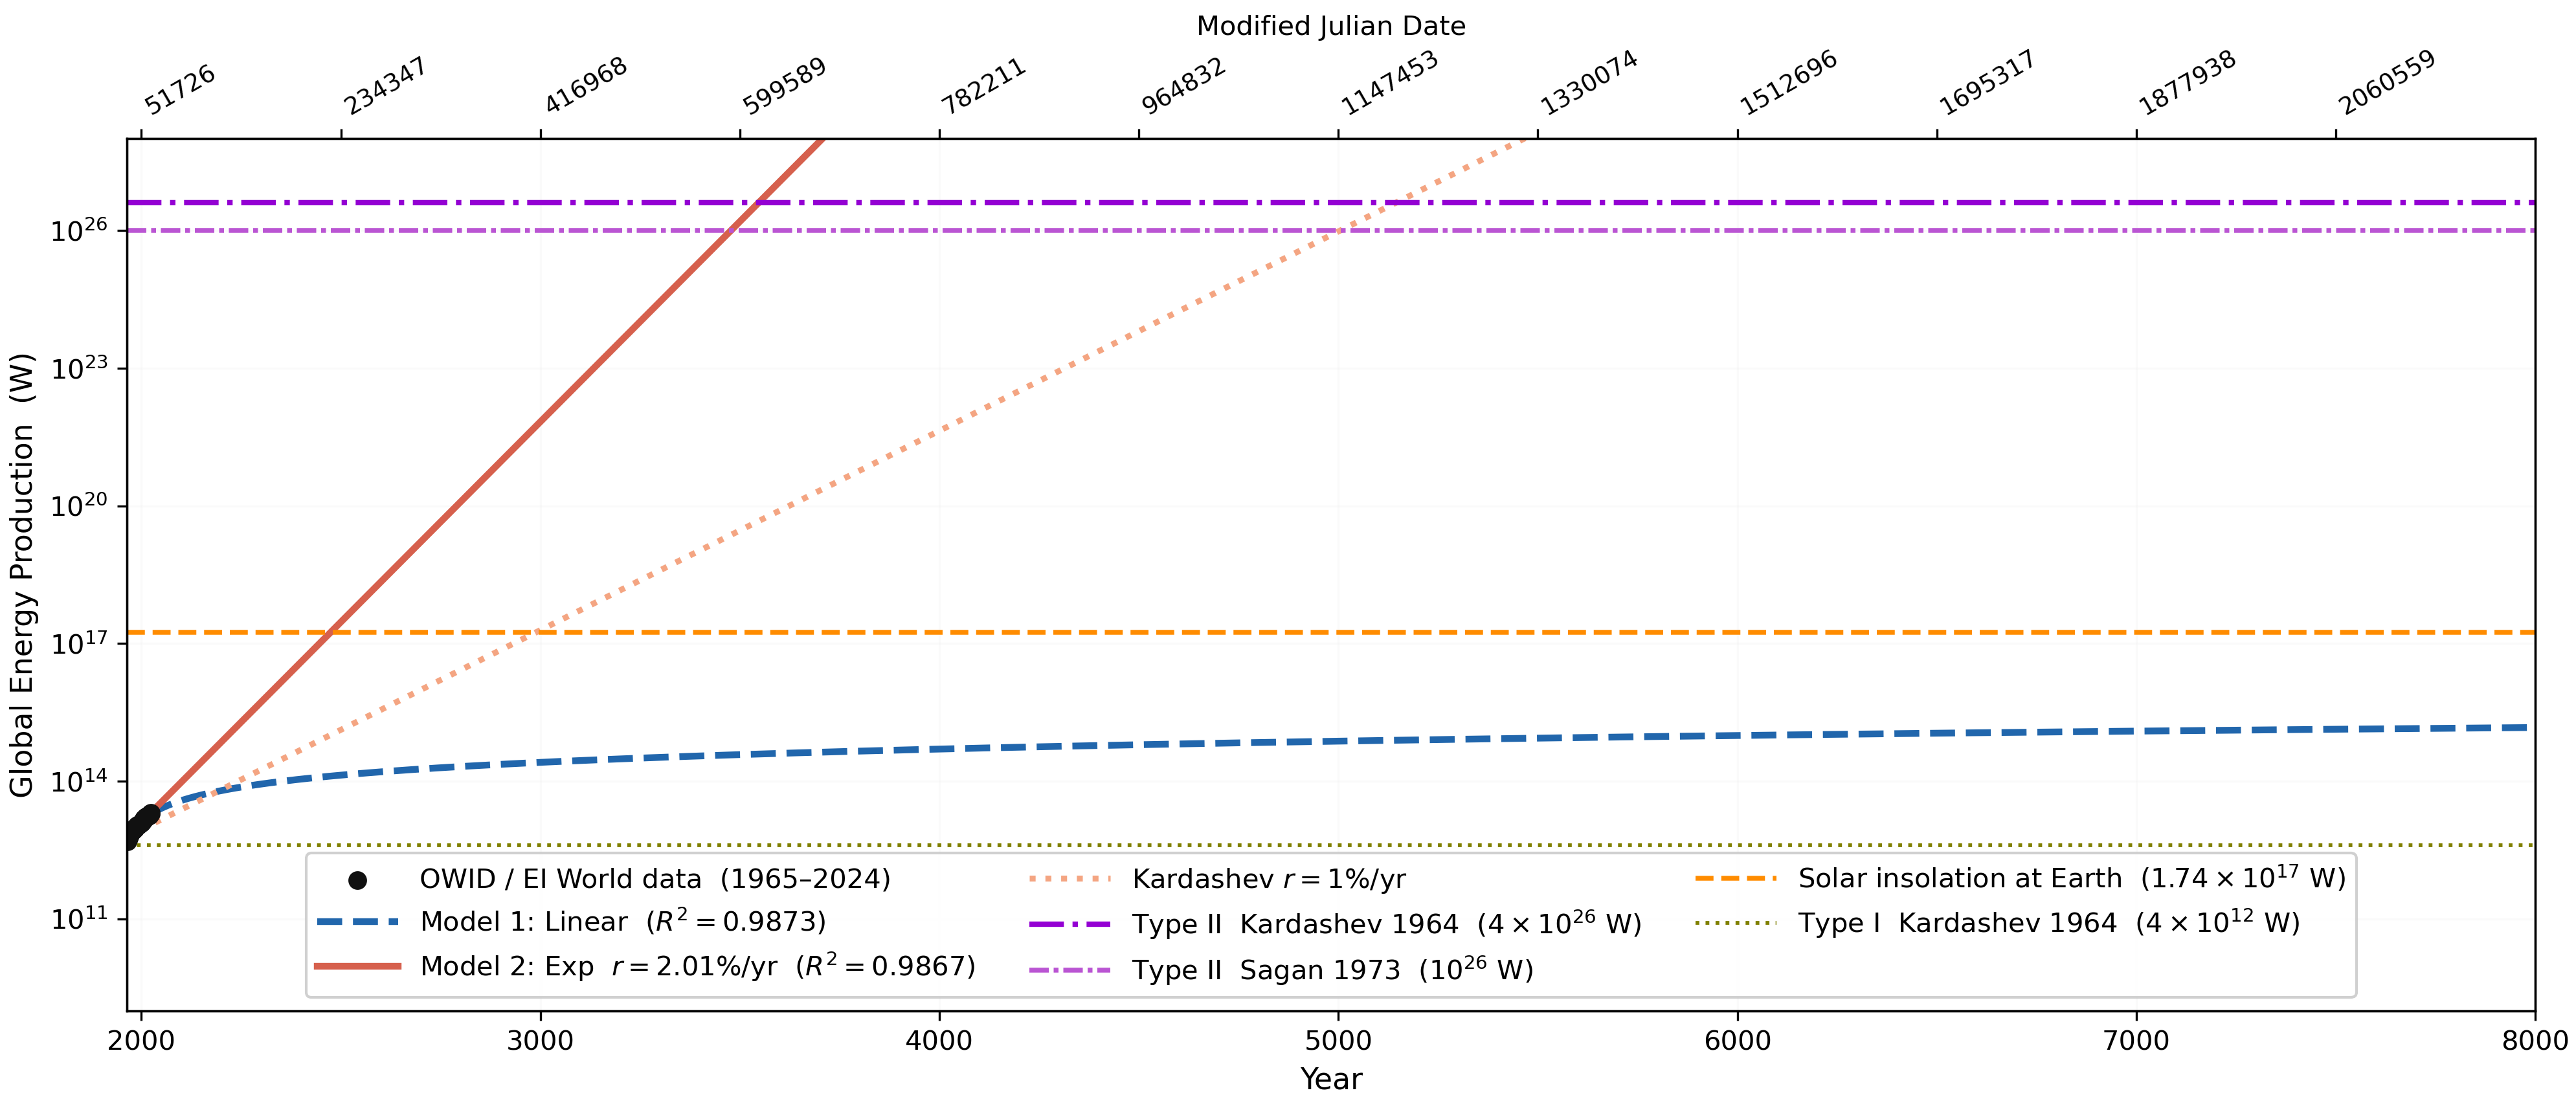
\includegraphics[width=\textwidth]{figs/KSN_panel1.png}
    \caption{Global energy production 1965--2024 (OWID dataset) in watts,
    with the standard Kardashev one-percent exponential model
    (dashed-orange), the best-fit linear OLS model (solid-red), and the
    Kardashev Type~I and Type~II civilisation thresholds (Horizontal lines).
    The Kardashev model diverge visibly from the OLS data fit over
    the full six-decade time baseline.}
    \label{fig:ksn_panel1}
\end{figure*}

\begin{figure}[t]
    \centering
    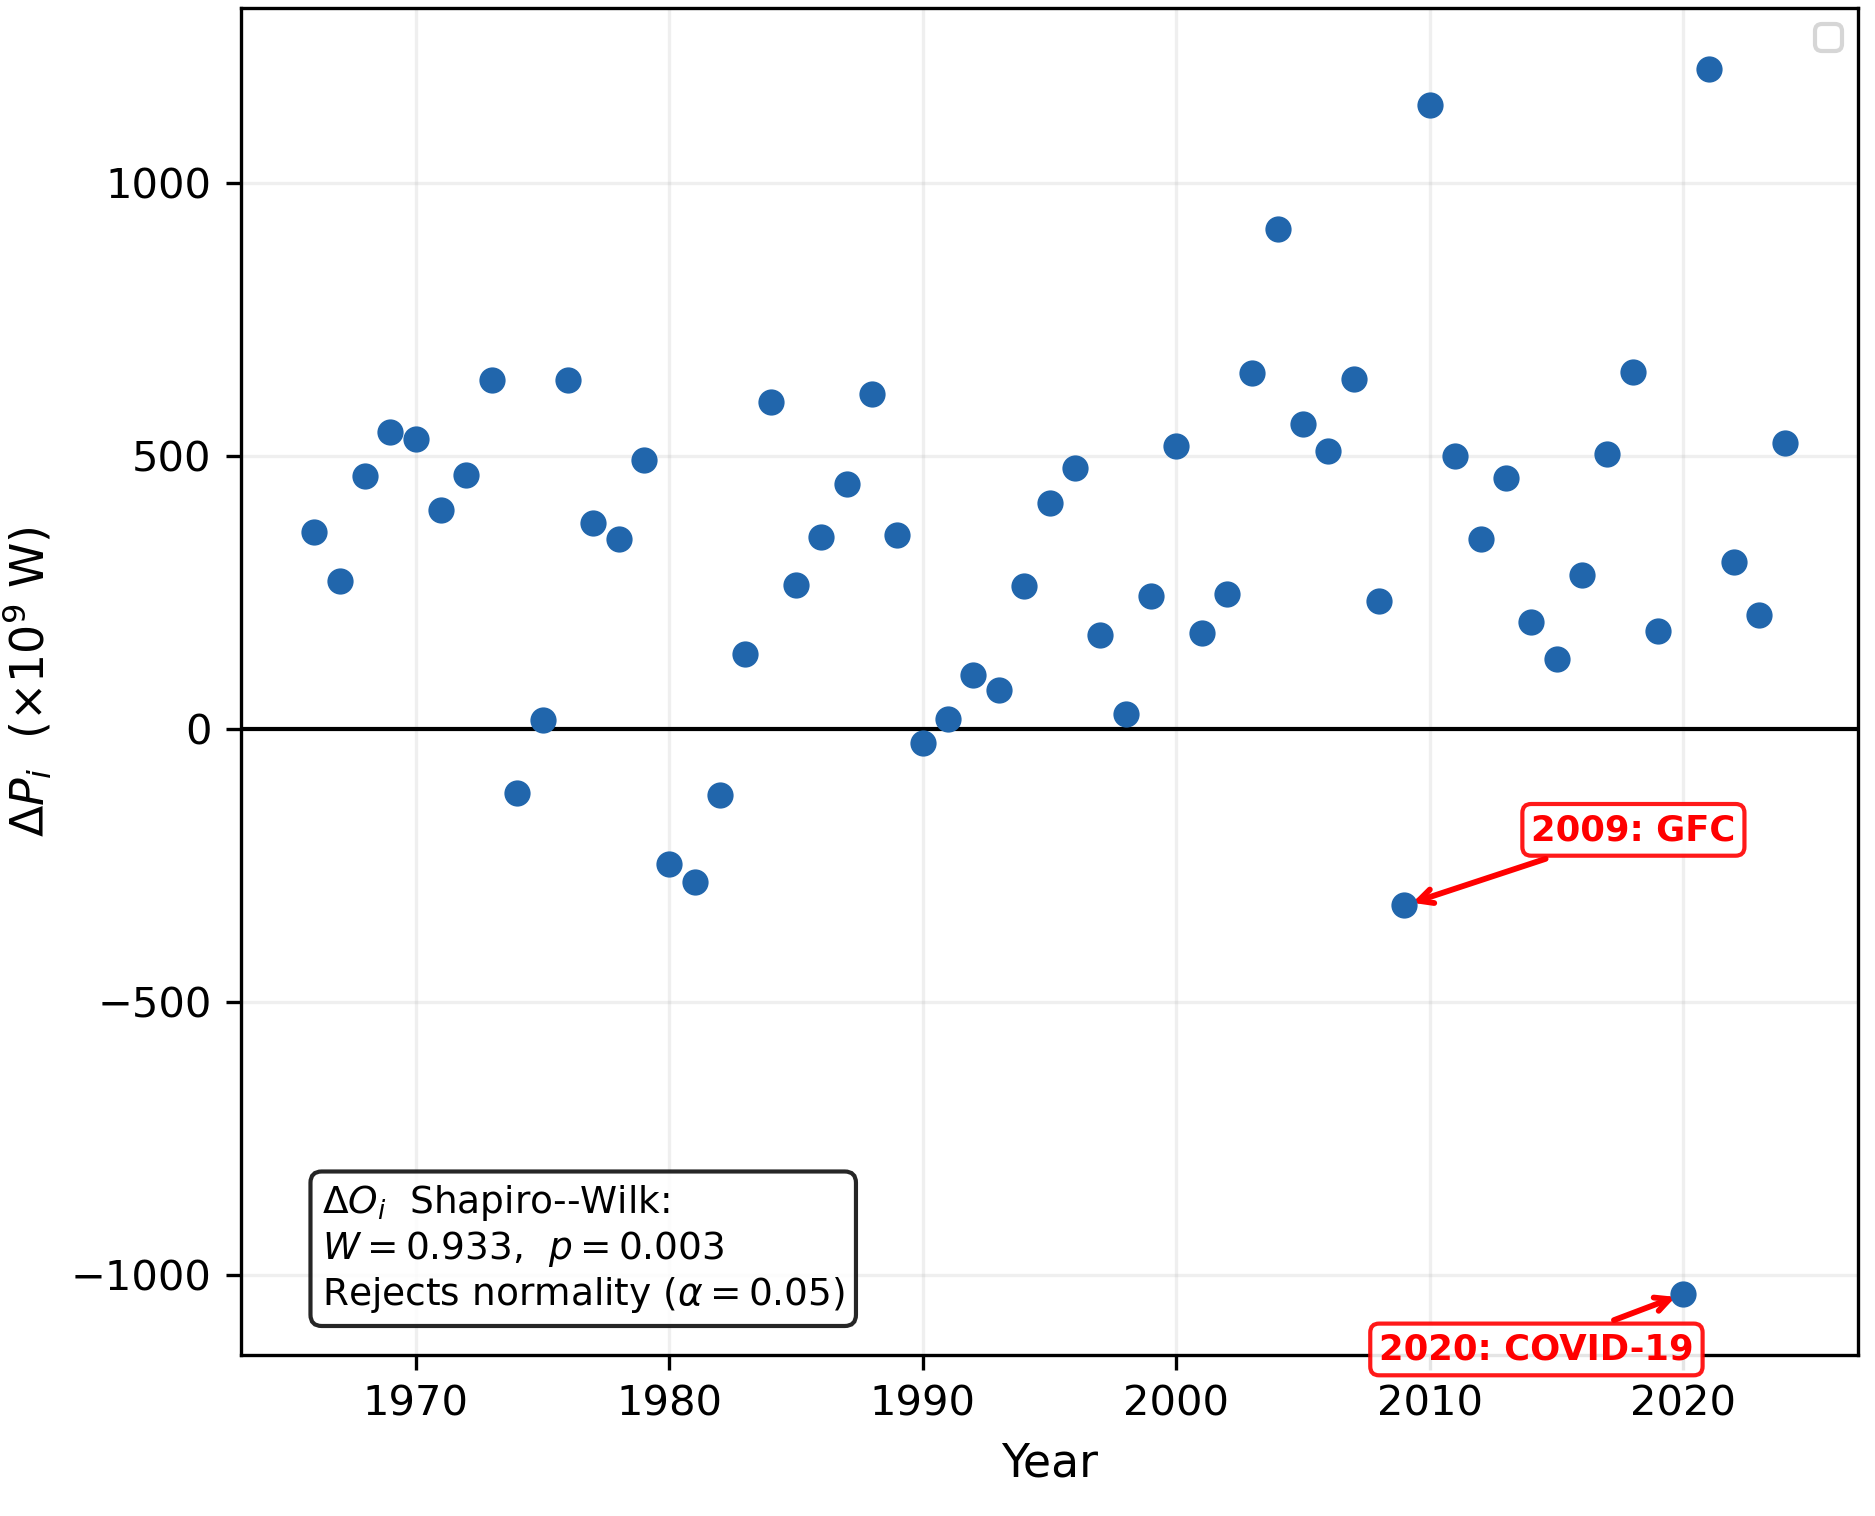
\includegraphics[width=\columnwidth]{figs/KSN_panel3.png}
    \caption{Distribution of year-over-year change in energy 
    $\Delta P = P_i - P_{i-1}$ (histogram), with a fitted
    normal distribution overlaid. The distribution is
    non-Gaussian and negatively skewed (Shapiro--Wilk
    $W = 0.925$, $p = 0.0014$), with the two largest
    negative outliers corresponding to the 2008 financial
    crisis and the 2020 COVID-19 pandemic.}
    \label{fig:ksn_panel3}
\end{figure}

\begin{figure}[t]
    \centering
    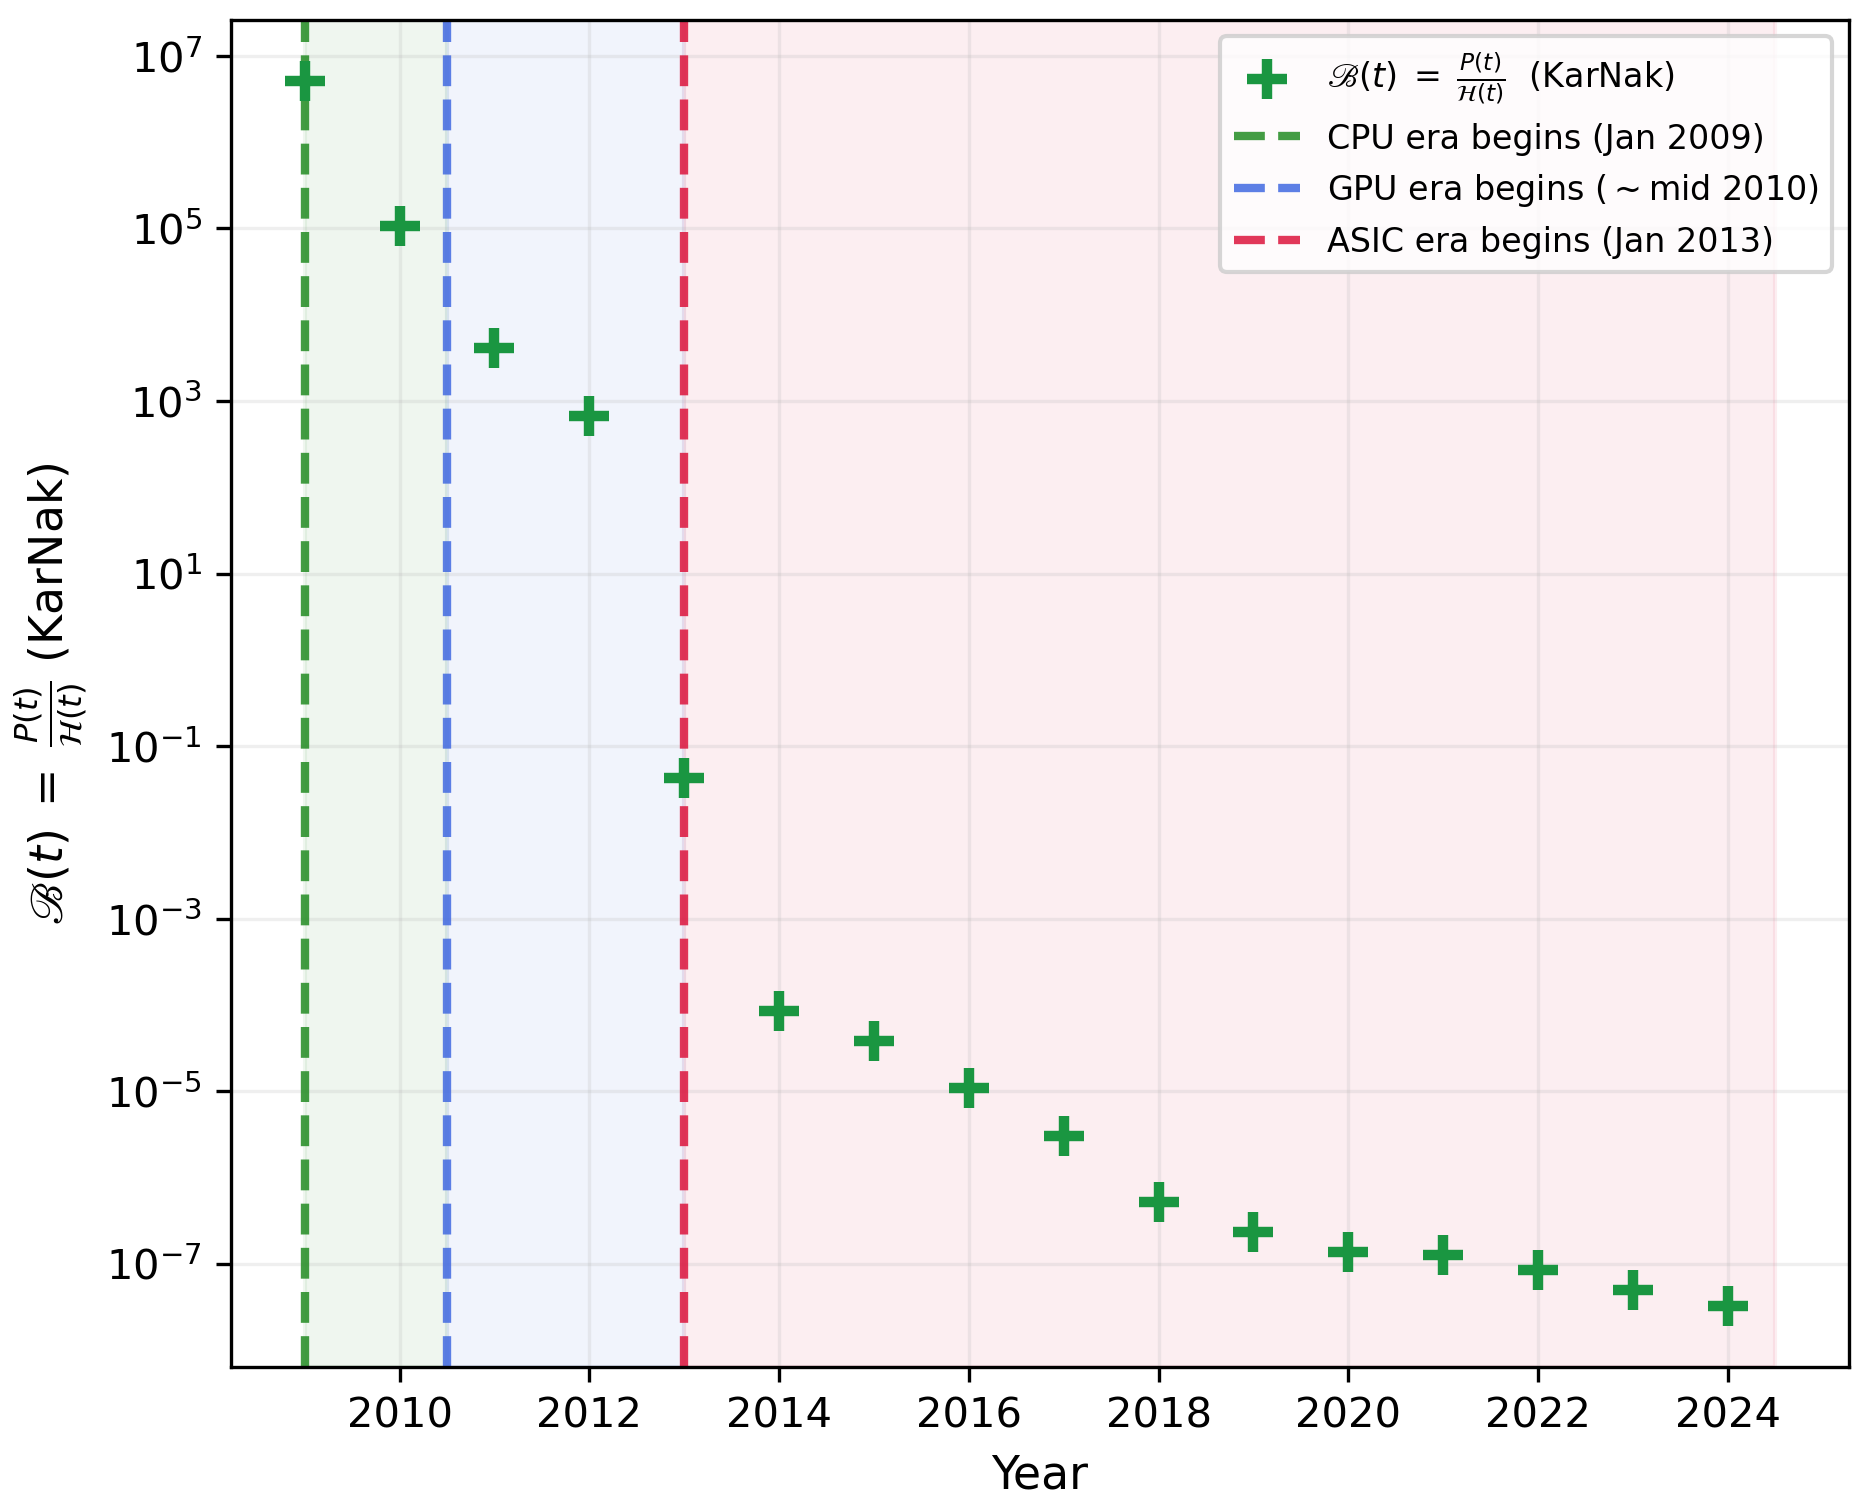
\includegraphics[width=\columnwidth]{figs/KSN_panel2.png}
    \caption{The KSN state variable $\mathscr{B}(t) = P(t)/\mathcal{H}(t)$
    in KarNak units (J\,Hash$^{-1}$) for 2009--2024,
    spanning 14 orders of magnitude. The monotonically
    decreasing trend reflects the rapid improvement in
    Bitcoin proof-of-work energy efficiency from the CPU
    era (2009) through the GPU era (2010--2012) to the
    ASIC era (2013--2024). Structural breaks between
    eras preclude a single-exponential description;
    a formal fit is deferred to a future paper.}
    \label{fig:ksn_panel2}
\end{figure}


\section{Discussion}
\label{sec:discussion}
 
\subsection{Falsifiability of the KSN Model}
 
A scientific model is meaningful only insofar as it generates
predictions that can in principle be refuted by data
\citep{Blumer1987}. We identify four concrete falsification
criteria for the KSN model.
 
First, the posterior growth rate $r = 2.01\% \pm 0.03\%\,
\mathrm{yr}^{-1}$ is a quantitative prediction: if sustained
observation of global energy production over the coming
decades yields a growth rate consistently outside the 95\%
credible interval $[1.94\%, 2.08\%]$, the exponential component
of the KSN framework is falsified.
 
Second, the non-Gaussian structure of $\Delta P$
(Shapiro--Wilk $W = 0.925$, $p = 0.0014$) establishes that
year-over-year energy increments exhibit path-dependent behaviour
driven by identifiable historical events. This is a testable
claim: if future decades produce a $\Delta P$ distribution
consistent with memoryless exponential growth, the path-dependence
argument is falsified.
 
Third, the KSN variable $\mathscr{B} = P/\mathcal{H}$ predicts a monotonically
decreasing trend as Bitcoin ASIC efficiency improves toward
the Landauer limit \citep{Landauer1961}. If the Bitcoin hashrate
growth stalls or reverses permanently --- for example if
proof-of-work mining becomes economically unviable --- the
KSN variable would cease to decrease and the renormalization
would lose its physical motivation. This is a genuine
falsification risk that the model acknowledges explicitly.
 
Fourth, the dimensional incompleteness argument predicts that
no functional form fitted to $P(t)$ alone can resolve
Kardashev's Conundrum. If a future author produces a model
of $P(t)$ without additional state variables that gives both
a statistically adequate fit to the data and a physically
coherent Type~II timescale, the KSN renormalization is
unnecessary and the argument is falsified.
 
\subsection{Limitations}
\label{sec:limitations}
 
Several limitations of the present analysis deserve explicit
acknowledgement.

A methodological choice concerns the energy accounting convention.
The OWID dataset column \texttt{primary\_energy\_consumption} reports
values using the direct primary energy method, which records the
physical energy output of each source. The alternative substitution
method inflates non-fossil contributions (nuclear, hydro, wind, solar)
by a thermal efficiency factor ($\sim 0.38$--$0.40$) to estimate the
fossil fuel input that would have produced the same electricity.
We adopt the direct method because the Kardashev scale measures
physical power, not fossil-fuel equivalents. We have verified that
all qualitative conclusions --- falsification of the one-percent
model, preference for the linear fit, and the persistence of the
Conundrum --- hold under the substitution method, with quantitative
differences: the substitution method yields $P(1965) = 7.66\,
\mathrm{TW}$, $b = 3.12 \times 10^{11}\,\mathrm{W\,yr}^{-1}$,
$r = 1.85\%\,\mathrm{yr}^{-1}$, and a Type~II timescale of
$\sim 8.9 \times 10^4\,H_0^{-1}$. The choice of accounting method
does not affect the dimensional incompleteness argument that motivates
the KSN renormalisation. We note that the distinction between these
methods will grow in significance as the global energy mix shifts
toward nuclear and renewable sources --- a transition that appears
to be accelerating, with several nations expanding nuclear capacity
--- since the substitution method increasingly overstates the total
energy budget relative to the physical power actually delivered.
 
The Bitcoin network hashrate is the only publicly auditable
global proof-of-work dataset currently available, but it
represents a single network. A more complete KSN state
variable would integrate all global computational
proof-of-work, including other proof-of-work cryptocurrencies
and, eventually, any future large-scale computational
infrastructure that provides an unforgeable public record.
The present analysis should therefore be understood as
a proof of concept using the best available proxy, rather
than a definitive measurement of civilisational
computational efficiency.
 
The hashrate data span only 2009--2024 --- sixteen annual
data points covering approximately one human generation.
The KSN variable exhibits structural breaks between the
CPU/GPU era (2009--2012) and the ASIC era (2013--2024),
reflecting qualitative changes in the technology of
proof-of-work computation rather than smooth continuous
evolution. A formal era-segmented fit to $\mathcal{H}(t)$ is deferred
to a future paper.
 
A further limitation concerns the production--consumption
distinction. The OWID dataset reports total primary energy
production, whereas \citet{kar64} defined his scale in terms
of energy \emph{consumption}. We have argued that production
constitutes a valid upper-limit proxy for consumption at
the civilisational scale, and that the two track each other
closely over decadal baselines. However, the ratio of
production to consumption is not precisely unity and varies
with time, introducing a systematic uncertainty that is
difficult to quantify without a separate long-baseline
consumption dataset. We note that our pull request to the
OWID energy repository \citep{owidenergy} identified and
documented this label inconsistency between the column name
\texttt{primary\_energy\_consumption} and the actual measured
quantity, which is production.
 
\subsection{The Novel Observation on Kardashev's Growth Rates}
 
A result that has received no attention in the literature
emerges directly from re-reading \citet{kar64}. Kardashev
presents \emph{two distinct growth rates} in the same paper:
an empirical estimate of $3$--$4\%\,\mathrm{yr}^{-1}$
based on statistical findings over the following sixty years,
and a conservative model assumption of $x = 1\%\,\mathrm{yr}^{-1}$
used for the Type~II timescale calculation. The standard
Kardashev model universally cited in the literature
\citep{gray2020} uses the conservative $1\%$ figure, not
Kardashev's own central estimate.
 
Our MCMC posterior growth rate of $r = 2.01\% \pm 0.03\%\,
\mathrm{yr}^{-1}$ lies closer to Kardashev's own empirical range
of $3$--$4\%\,\mathrm{yr}^{-1}$ than to his conservative $1\%$
assumption, and well above the standard one-percent model.
This is not a falsification of \citet{kar64}; it is a vindication
of his empirical judgment. The standard ``one-percent Kardashev
model'' is falsified not because Kardashev was wrong, but
because the literature has universally adopted his deliberately
conservative lower bound rather than his actual empirical
estimate.
 
\subsection{Connection to the Drake Equation}
 
The Drake equation for the number of communicating
civilisations in the Galaxy includes a longevity factor $L$
--- the average duration for which a civilisation remains
detectable. This factor carries the largest relative
uncertainty of any term in the Drake equation and is
sensitive to whether civilisations tend to self-destruct
or achieve long-term stability \citep{gray2020}.
 
The KSN model is relevant to the longevity factor in the
following sense: a civilisation that approaches the Landauer
limit --- that is, one for which $\mathscr{B} \to k_B T \ln 2$ per
bit --- has achieved near-optimal use of available energy
for computation, which we argue is a necessary condition
for long-term civilisational stability. The KSN Type~II
threshold, defined as $\mathscr{B}$ approaching the Landauer limit,
is therefore not merely an energy milestone but an
information-thermodynamic one. Whether $L$ is large or
small may depend on whether civilisations reach this
threshold before exhausting or destabilising their energy
resources --- a question the KSN model frames quantitatively
for the first time.
 
\subsection{The Doomsday Clock}
 
The Bulletin of the Atomic Scientists advanced the
Doomsday Clock to 85 seconds to midnight in 2026 ---
the closest it has been to civilisational catastrophe in
the history of the index. The KSN model provides an
independent quantitative perspective on civilisational
risk: the dramatic decrease in $\mathcal{H}(t)$ observed over
2009--2024 reflects an exponential improvement in the
energy efficiency of global computation, consistent with
a civilisation moving \emph{toward} the Landauer limit.
Whether this trajectory can be sustained, and whether
it will be accompanied by the institutional stability
required to avoid catastrophe, lies beyond the scope of
this model --- but the KSN framework provides the
quantitative language in which such questions can
eventually be posed. We note that in his 1985
congressional testimony on climate change,
\citet{Sagan1985} identified the need for ``a degree of
international amity which certainly doesn't exist today.''
We speculate that decentralised proof-of-work protocols,
by providing trustless cooperation without requiring
political goodwill, may offer a partial technological
foundation for the amity Sagan envisioned.

\section{Conclusions}
\label{sec:conclusions}
 
We have tested the standard Kardashev one-percent exponential
model against six decades of global energy production data
and found it statistically untenable. The posterior growth
rate from MCMC inference is $r = 2.01\% \pm 0.03\%\,
\mathrm{yr}^{-1}$ (95\% credible interval $[1.94\%, 2.08\%]$),
placing the Kardashev one-percent value well outside the
credible interval. The year-over-year energy differences exhibit
significant non-Gaussian, path-dependent structure
(Shapiro--Wilk $W = 0.925$, $p = 0.0014$), with negative
skewness attributable to identifiable crisis events (2008, 2020),
incompatible with the memoryless multiplicative structure
required by any exponential growth model.
 
A linear OLS model fits the data excellently ($R^2 = 0.987$)
and is marginally preferred over the free-parameter exponential
model by the Widely Applicable Information Criterion
($\Delta\mathrm{WAIC} = 5.5$). However, extrapolation of the
linear model to the Kardashev Type~II threshold yields a
civilisational transition timescale of $\sim 1.2 \times 10^5$
Hubble times --- a physical reductio ad absurdum we term
\textit{Kardashev's Conundrum}. No functional form fitted
to energy production alone can simultaneously satisfy
statistical adequacy and physical coherence, because the
Kardashev state variable is dimensionally incomplete as
a measure of civilisational advancement.
 
We have proposed the Kardashev--Sagan--Nakamoto (KSN)
model as a resolution: renormalising the energy production
ordinate by the annual average Bitcoin network hashrate
$\mathcal{H}(t)$, yielding the KSN state variable $\mathscr{B}(t) \;=\; \frac{P(t)}{\mathcal{H}(t)}$ in
units of J\,Hash$^{-1}$ --- the KarNak unit. This
renormalisation adds no free parameters, is physically
motivated by the Landauer limit connecting energy to
irreversible computation \citep{Landauer1961}, and fulfils
the requirement of \citet{sagan73} that the Kardashev
scale be sensitive to the information richness of a
civilisation. The KSN variable spans 14 orders of magnitude
over 2009--2024, tracing the trajectory of energy-to-computation
efficiency from the CPU era through to modern ASICs.
 
We further note, for the first time in the literature, that
\citet{kar64} presented two distinct growth rates: an
empirical estimate of $3$--$4\%\,\mathrm{yr}^{-1}$ and a
conservative model assumption of $1\%\,\mathrm{yr}^{-1}$.
Our posterior $r = 2.01\%\,\mathrm{yr}^{-1}$ lies closer to
Kardashev's own empirical range, vindicating his empirical
judgment while definitively falsifying the conservative
assumption that the literature has universally adopted as
the standard model.
 
A formal era-segmented functional fit to $\mathcal{H}(t)$, accounting
for the structural breaks between the CPU, GPU, and ASIC
eras of Bitcoin mining, is deferred to a future work. The
KarNak unit is proposed as a universal information-energy
yardstick for the Kardashev scale, and the KSN framework
as a quantitative language for discussing civilisational
longevity in the context of the Drake equation.
 

% =============================================================================
% SECTION Declarative AI
% =============================================================================
\section*{Declaration of Generative AI and AI-assisted technologies in the writing process}
During the preparation of this work the author used Claude (Anthropic) in order to
assist with statistical verification, code debugging, dimensional analysis, and
manuscript editing. After using this tool, the author reviewed and edited the
content as needed and takes full responsibility for the content of the publication.

% =============================================================================
% SECTION Acknowledgments
% =============================================================================
\section{Acknowledgments}
SG thanks R. Gamen from the VO of Argentina (NOVA) for the opportunity to serve as Argentina's representative on the IVOA Executive Committee (2015–2024), and C. Cui (National Astronomical Observatories, CAS) for encouragement during the preparation of this work. SG also thanks colleagues at the IATE and the OAC for their support. This work made use
of Astropy, a community-developed core Python package for
Astronomy \citep{robitaille_astropy:_2013}, and the broader
open-source scientific software ecosystem stack including SciPy and
NumPy.Simulations were run on the Sersic
cluster at the `Instituto de Astronomía Teórica y Experimental' (IATE).This research was partially conducted during a period of unpaid leave 
from CONICET, the Astronomical Observatory of C\'ordoba and the National University of C\'ordoba, 
motivated by national government austerity measures that suspended research funding across Argentine scientific institutions.
 
\noindent\textbf{Author contributions (CRediT):}
S.~Gurovich: Conceptualization, Methodology, Software,
Formal analysis, Investigation, Writing -- original draft,
Writing -- review \& editing, Visualization,
Project administration.

% =============================================================================
% SECTION BIBLIO
% =============================================================================
%
%\section*{References}
%\label{biblio}
% Astronomy and Computing (Elsevier) uses the elsarticle Harvard (author–year) style.
\bibliographystyle{elsarticle-harv}
\bibliography{astroblock}


\end{document}

\endinput